\documentclass[conference]{IEEEtran}
\IEEEoverridecommandlockouts
% The preceding line is only needed to identify funding in the first footnote. If that is unneeded, please comment it out.
\usepackage{cite}
\usepackage{amsmath,amssymb,amsfonts}
\usepackage{algorithmic}
\usepackage{graphicx}
\usepackage{array}
\usepackage{textcomp}
\usepackage[table]{xcolor} 12345
\usepackage{multirow}
\usepackage{multicol}
\usepackage{float}
\usepackage[utf8]{inputenc}
\usepackage[vietnamese]{babel}
\usepackage{amsmath}
\def\BibTeX{{\rm B\kern-.05em{\sc i\kern-.025em b}\kern-.08em
    T\kern-.1667em\lower.7ex\hbox{E}\kern-.125emX}}
\documentclass{article}
\title{Sử dụng kỹ thuật phân tích Chuỗi thời gian vào bài toán dự đoán giá Cổ phiếu}
\author{\IEEEauthorblockN{1\textsuperscript{st} Nông Tiến Dũng}
\IEEEauthorblockA{\textit{{IS304.O21.VN}} \\
\textit{Đại học Công nghệ Thông tin}\\
20521213@gm.uit.edu.vn}
\and
\IEEEauthorblockN{2\textsuperscript{nd} Đỗ Văn Sáng}
\IEEEauthorblockA{\textit{IS304.O21.VN} \\
\textit{Đại học Công nghệ Thông tin}\\
20521832@gm.uit.edu.vn}
\and
\IEEEauthorblockN{3\textsuperscript{rd} Tạ Quang Hưng}
\IEEEauthorblockA{\textit{IS304.O21.VN} \\
\textit{Đại học Công nghệ Thông tin}\\
21520036@gm.uit.edu.vn}
\and
\IEEEauthorblockN{4\textsuperscript{th} La Hoài Nam}
\IEEEauthorblockA{\textit{IS304.O21.VN} \\
\textit{Đại học Công nghệ Thông tin}\\
20521629@gm.uit.edu.vn}
\and
\IEEEauthorblockN{5\textsuperscript{th} Nguyễn Quang Huy}
\IEEEauthorblockA{\textit{IS304.O21.VN} \\
\textit{Đại học Công nghệ Thông tin}\\
20521403@gm.uit.edu.vn}
}
\begin{document}
\maketitle

\begin{abstract}
Bài báo sử dụng kỹ thuật phân tích chuỗi thời gian trong bài toán dự đoán giá cổ phiếu. Dự đoán giá cổ phiếu là một tác vụ khó khăn do tính phức tạp và biến động của thị trường tài chính. Trong bài báo, chúng tôi sử dụng các mô hình: Exponential Smoothing State Space Model (ETS), Meta-Learning, Fuzzy for predict times series, LightGBMModel, ResCNN, Linear regression, Autoregressive Integrated Moving Average (ARIMA), Recurrent Neural Networks (RNN), Gated recurrent units (GRU), và Long Short-Term Memory (LSTM) để dự đoán giá cổ phiếu trên ba bộ dữ liệu AbbVie, AstraZeneca và Pfizer. Sau đó thực hiện so sánh hiệu suất của các mô hình dựa trên ba độ đo: RMSE, MAE và MAPE.
\end{abstract}

\begin{IEEEkeywords}
Cổ phiếu, ETS, Meta-Learning, Fuzzy for predict times series, LightGBMModel, ResCNN, Linear regression, ARIMA, RNN, GRU, LTSM
\end{IEEEkeywords}

\section{GIỚI THIỆU}
Cổ phiếu được coi là hình thức đầu tư trọng điểm trong ngành tài chính, đại diện cho quyền sở hữu một phần trong tổ chức phát hành. Theo Investopedia, công ty Đông Ấn Hà Lan phát hành cổ phiếu đầu tiên vào năm 1602 tại Sở Giao dịch Chứng khoán Amsterdam, đồng thời cũng là công ty đầu tiên phát hành cổ phiếu và trái phiếu. Điều này đã được coi là một sự tiến bộ quan trọng trong lĩnh vực tài chính và đã mở ra thời kỳ phát triển của thị trường cổ phiếu.

Định giá cổ phiếu là quy trình xác định giá trị thị trường thực sự của cổ phiếu tại một thời điểm nhất định, nhằm hiểu rõ tiềm năng của cổ phiếu để đưa ra quyết định đầu tư phù hợp. Đối với doanh nghiệp, việc định giá cổ phiếu được coi là một trong những bước tiên quyết khi công ty cổ phần dự định phát hành cổ phiếu, huy động vốn và tăng cường ảnh hưởng của mình trên thị trường. Từ góc độ của nhà đầu tư, việc định giá cổ phiếu giúp họ xác định cổ phiếu nào đáng để đầu tư và có tiềm năng mang lại lợi nhuận tối đa.

Một phương pháp tiếp cận sơ bộ trong việc định giá cổ phiếu là đánh giá giá trị cổ phiếu. Nếu giá cổ phiếu hiện tại thấp hơn giá trị đã định giá, nhà đầu tư có thể xem xét mua cổ phiếu. Ngược lại, nếu giá cổ phiếu vượt quá giá trị đã định giá và nhà đầu tư hiện đang sở hữu cổ phiếu, họ có thể bán cổ phiếu để thu về lợi nhuận.

Thực tế cho thấy có nhiều thuật toán và kỹ thuật hỗ trợ việc dự báo giá cổ phiếu của ba doanh nghiệp bao gồm: Catalent, Intel Corporation, Nutrien. Trong nghiên cứu này, chúng tôi sẽ áp dụng 10 mô hình: Exponential Smoothing State Space Model (ETS), Meta-Learning, Fuzzy for predict time series, LightGBMModel, ResCNN, Linear regression, ARIMA, RNN, GRU, LSTM để tiến hành đánh giá hiệu suất các mô hình, sau đó sử dụng hai mô hình tốt nhất thực hiện dự đoán giá đóng cửa của cổ phiếu trong 30 ngày, 60 ngày và 90 ngày tiếp theo. 

\section{CÁC NGHIÊN CỨU LIÊN QUAN}
Zou Xiaowu và đồng nghiệp cung cấp các phương pháp dựa trên CNN cho Phân loại Chuỗi Thời gian (TSC) [1] và các hàm kích hoạt được sử dụng. Một MC-CNN được đề xuất cho phân loại chuỗi thời gian đa biến. Phương pháp này trích xuất đặc trưng bằng cách sử dụng nhiều CNN khác nhau và kết hợp chúng. một CNN đa quy mô.

Guolin Ke và đồng nghiệp đề xuất hai kỹ thuật mới là Gradient-based One-Side Sampling (GOSS) và Exclusive Feature Bundling (EFB). GOSS tập trung vào việc loại bỏ một phần lớn các mẫu dữ liệu có độ dốc thấp, trong khi EFB gom nhóm các đặc trưng phân biệt để giảm số lượng đặc trưng. Cả hai kỹ thuật này nhằm tối ưu hóa hiệu suất huấn luyện của GBDT và giảm thiểu thời gian tính toán [2].

European Centre for Medium-Range Weather Forecasts (ECMWF) sử dụng mô hình EMOS để cải thiện dự báo thời tiết từ mô hình dự báo số học [3]. Việc áp dụng EMOS đã giúp ECMWF cải thiện độ chính xác của dự báo thời tiết, đặc biệt là ở các kỳ vọng ngắn và trung hạn.

Nhóm Simon J. Julier và Jeffrey K. Uhlmann[4] đã nghiên cứu phần mở rộng mới của thuật toán Kalman Filter (EKF) để xử lý các hệ thống phi tuyến. Họ đã sử dụng dữ liệu về phương tiện đi vào khí quyển với độ cao lớn. Kết quả mô hình cho thấy unscented filter ước tính sai số bình phương trung bình của nó rất chính xác và có thể tin tưởng vào các ước tính của bộ lọc. Tuy nhiên, EKF rất không nhất quán: sai số bình phương trung bình cực đại trong x1 là 0,4km2 trong khi hiệp phương sai ước tính của nó nhỏ hơn một trăm lần. Phần mở rộng của thuật toán Kalman Filter này loại bỏ hiệu quả hầu hết các phép biến đổi tọa độ phi tuyến thông thường.

Trong một nghiên cứu được công bố vào năm 2007, Chin-Teng Lin và đồng nghiệp đã sử dụng mô hình Fuzzy Time Series để dự đoán huyết áp trong tương lai dựa trên các giá trị huyết áp trong quá khứ [5]. Mô hình này sử dụng các tập luật Fuzzy để mô hình hóa mối quan hệ giữa các biến số đầu vào và đầu ra. Kết quả của nghiên cứu cho thấy rằng mô hình Fuzzy có khả năng dự đoán chuỗi thời gian của huyết áp một cách chính xác và hiệu quả, giúp trong việc theo dõi sức khỏe của bệnh nhân và đưa ra các biện pháp phòng ngừa kịp thời.

Nhóm tác giả Vaishnavi Gururaj, Shriya V R và Dr. Ashwini K [6] đã nghiên cứu về thị trường chứng khoán bằng mô hình Linear Regression. Dataset mà nhóm tác giả sử dụng là một năm dữ liệu cổ phiếu của Công ty Coca-Cola, từ 01/2017-2018. Các kết quả về độ đo bao gồm: 3.22 (RMSE), 2.53 (MAE), 10.37 (MSE) và 0.73 (R-Squared).

Nghiên cứu "Performance analysis of machine learning models for intrusion detection system using Gini Impurity-based Weighted Random Forest (GIWRF) feature selection technique"[7], tác giả Raisa Abedin Disha và S. Waheed đã thử nghiệm và đánh giá hiệu suất của các mô hình học máy như GRU và GBT trong việc phân loại trong hệ thống phát hiện xâm nhập. Các mô hình này đã được huấn luyện và kiểm tra trên hai tập dữ liệu UNSW-NB 15 và Network TON\_IoT. Để tăng cường hiệu suất của các mô hình, tác giả đã sử dụng kỹ thuật lựa chọn đặc trưng gọi là Gini Impurity-based Weighted Random Forest (GIWRF). Kỹ thuật này giúp tác giả chọn ra một tập hợp tối ưu các đặc trưng từ dữ liệu. Kết quả thực nghiệm cho thấy mô hình Cây quyết định (DT) hoạt động tốt hơn so với các mô hình khác trong thí nghiệm này khi sử dụng kỹ thuật lựa chọn đặc trưng GIWRF.

Box và Jenkins đã giới thiệu mô hình ARIMA vào năm 1970. Đây còn được gọi là phương pháp Box-Jenkins, bao gồm một tập hợp các hoạt động để xác định, ước lượng và chẩn đoán các mô hình ARIMA với dữ liệu chuỗi thời gian [8]. Các mô hình ARIMA đã chứng minh khả năng tạo ra dự đoán ngắn hạn hiệu quả. ARIMA liên tục vượt trội so với các mô hình phức tạp khác trong dự đoán ngắn hạn [9].

Ba tác giả Murtaza Roondiwala, Harshal Patel và Shraddha Varma đã áp dụng mô hình LSTM (Long Short-Term memory) trong việc dự đoán giá trị của cổ phiếu của NIFTY 50 [10]. Họ đã sử dụng 500 epochs để train và kết quả đạt được là vô cùng tốt. Mô hình cho ra được các kết quả RMSE trên tập test rơi vào khoảng 0.00859. Sai số vô cùng thấp cho thấy giá trị dự đoán cực kì tốt.

Tác giả Yongqiong Zhu [11] đã sử dụng mô hình RNN để dự đoán giá cố phiếu của Apple với dữ liệu huấn luyện là giá cổ phiểu của Apple (AAPL) trong 10 năm (từ 9/8/2009 đến 12/8/2020 với tập train chiếm 65\% và tập test chiếm 35\% còn lại. Tác giả đã xây dựng mô hình mạng RNN hai lớp với lớp thứ nhất có 50 nút đơn vị và lớp thứ hai chứa 100 nút đơn vị. Tác giả sử dụng 50 epochs, tối ưu hóa bằng Adam và dùng hàm mất mát là MSE đã cho ra được một kết quả rất tốt. Mô hình cho kết quả độ chính xác của dự đoán lên đến hơn 95\% và giá trị mất mát là 0.1\%.

\section{TÀI NGHUYÊN}
\subsection{DỮ LIỆU}
Bài báo sử dụng bộ dữ liệu được lấy từ dữ liệu chứng khoán của 3 công ty ABBV (Dữ liệu của công ty AbbVie được lấy về từ trang web finance.yahoo.com có 1259 dòng dữ liệu), AZN (Dữ liệu của công ty AstraZeneca được lấy về từ trang web finance.yahoo.com có 1259 dòng dữ liệu) và PFE (Dữ liệu của công ty Pfizer được lấy về từ trang web finance.yahoo.com có 1259 dòng dữ liệu). Với dữ liệu được thu thập từ ngày 1/3/2019 đến ngày 29/2/2024 và được tải về vào ngày 14/4/2024. Ở cả 3 bộ dữ liệu đều có các cột thuộc tính liên quan đến cổ phiếu.

\begin{table}[H]
  \centering
  \caption{Mô tả thuộc tính trong ba bộ dữ liệu}
\begin{tabular}{|>{\columncolor{red!20}}c|c|}
    \hline
     \rowcolor{red!20} Thuộc tính & Mô tả\\ \hline
     Date & Ngày diễn ra giao dịch \\ \hline
     Open & Giá cổ phiếu đầu tiên được giao dịch\\ \hline
     High & Giá cao nhất của cổ phiếu được giao dịch\\ \hline
     Low & Giá thấp nhất của cổ phiếu được giao dịch\\ \hline
     Close & Giá đóng cửa của cổ phiếu\\ \hline
     Adj Close & Giá đóng của điều chỉnh\\ \hline
     Volume & Khối lượng giao dịch\\ \hline
\end{tabular}
\end{table}

Thông tin dữ liệu thu thập được mô tả chi tiết trong bảng 2. Bảng 2 thể hiện đánh giá tổng quan trên thuộc tính Close – Thuộc tính được lựa chọn để thực hiện dự đoán giá đóng cửa cổ phiếu.

\begin{table}[H]
  \centering
  \caption{Mô tả chi tiết về dữ liệu thu thập}
\begin{tabular}{|>{\columncolor{red!20}}c|c|c|c|}
    \hline
     \rowcolor{red!20} & ABBV & AZN & PFE\\ \hline
     Count & 1259 & 1259 & 1259 \\ \hline
     Mean & 118.409 & 57.12 & 39.942\\ \hline
     Std & 30.792 & 9.482 & 7.166\\ \hline
     Min & 62.98 & 37.28 & 26.13\\ \hline
     Max & 178.99 & 75.81 & 61.25\\ \hline
     25\% & 89.475 & 50.06 & 34.942\\ \hline
     50\% & 115.61 & 57 & 38.63\\ \hline
     75\% & 147.505 & 65.595 & 44.71\\ \hline
     Skewness & -0.027 & -0.176 & 0.54\\ \hline
     Kurtosis & -1.34 & -0.862 & -0.42\\ \hline
\end{tabular}
\end{table}
\begin{figure}[H]
    \centering
    \begin{minipage}{0.23\textwidth}
    \centering
    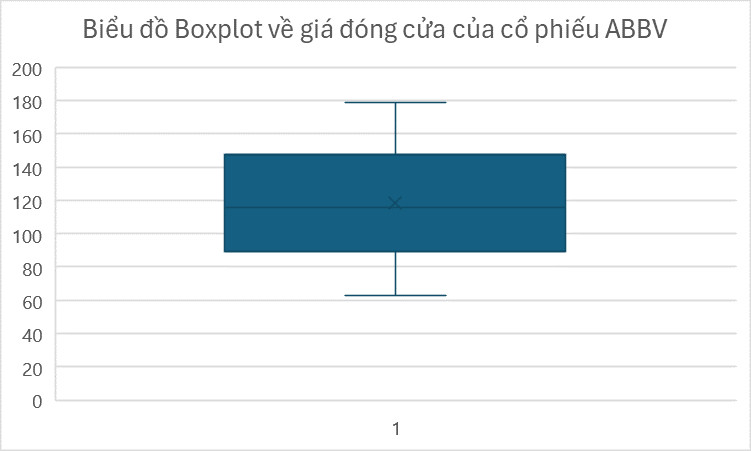
\includegraphics[width=1\textwidth]{Image/ABBV_Boxplot.jpg}
    \caption{Biểu đồ Box Plot giá đóng cửa của ABBV}
    \label{fig:1}
    \end{minipage}
    \hfill
    \begin{minipage}{0.23\textwidth}
    \centering
    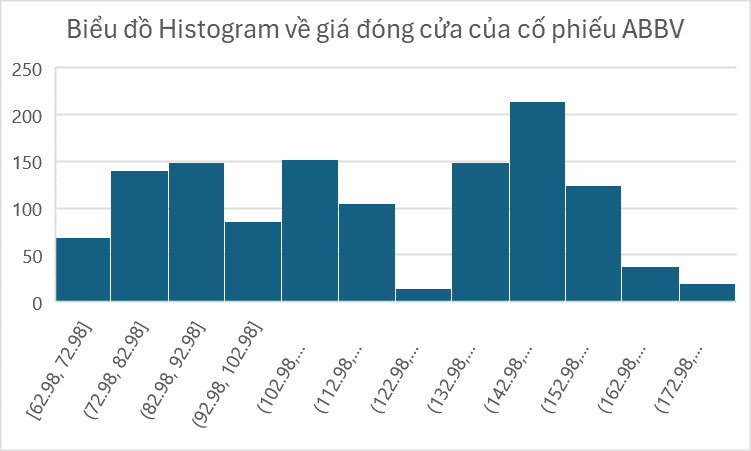
\includegraphics[width=1\textwidth]{Image/ABBV_Histogram.jpg}
    \caption{Biểu đồ Histogram giá đóng cửa của ABBV}
    \label{fig:2}
    \end{minipage}
\end{figure}
- Giá trị Skewness gần bằng 0 cho thấy phân phối dữ liệu có hình dạng gần đối xứng.

- Giá trị Kurtosis âm phân phối có độ nhọn thấp hơn bình thường

- Biểu đồ Histogram cho thấy tần suất xuất hiện của giá cổ phiếu có giá trị từ 142.98 đến 152.98 là nhiều nhất.

- Biểu đồ Boxplot cho thấy dữ liệu cổ phiếu ABBV không có giá trị ngoại lai và độ phân tán lớn.
\begin{figure}[H]
    \centering
    \begin{minipage}{0.23\textwidth}
    \centering
    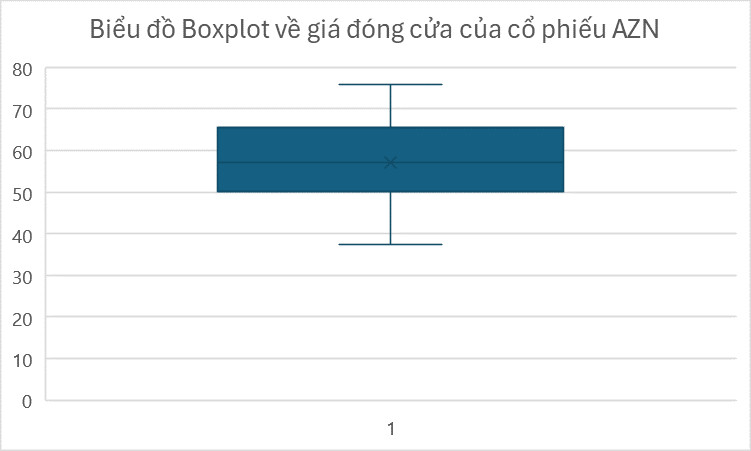
\includegraphics[width=1\textwidth]{Image/AZN_Boxplot.jpg}
    \caption{Biểu đồ Box Plot giá đóng cửa của AZN}
    \label{fig:1}
    \end{minipage}
    \hfill
    \begin{minipage}{0.23\textwidth}
    \centering
    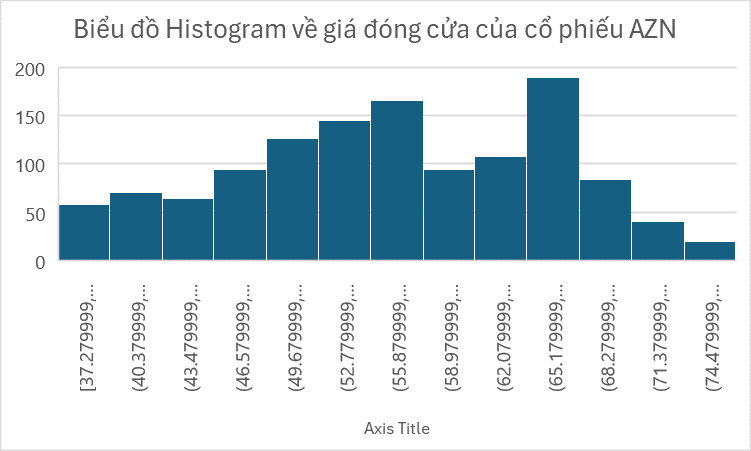
\includegraphics[width=1\textwidth]{Image/AZN_Histogram.jpg}
    \caption{Biểu đồ Histogram giá đóng cửa của AZN}
    \label{fig:2}
    \end{minipage}
\end{figure}
- Giá trị Skewness âm cho thấy phân phối dữ liệu lệch mạnh về bên trái so với trung vị.

- Giá trị Kurtosis âm tuy nhiên không có sự khác biệt lớn nên có độ nhọn thấp hơn bình thường.

- Biểu đồ Histogram cho thấy tần suất xuất hiện của giá cổ phiếu có giá trị từ 65.18 đến 68.28 là nhiều nhất.

- Biểu đồ Boxplot cho thấy dữ liệu cổ phiếu AZN không có giá trị ngoại lai và độ phân tán ít.
\begin{figure}[H]
    \centering
    \begin{minipage}{0.23\textwidth}
    \centering
    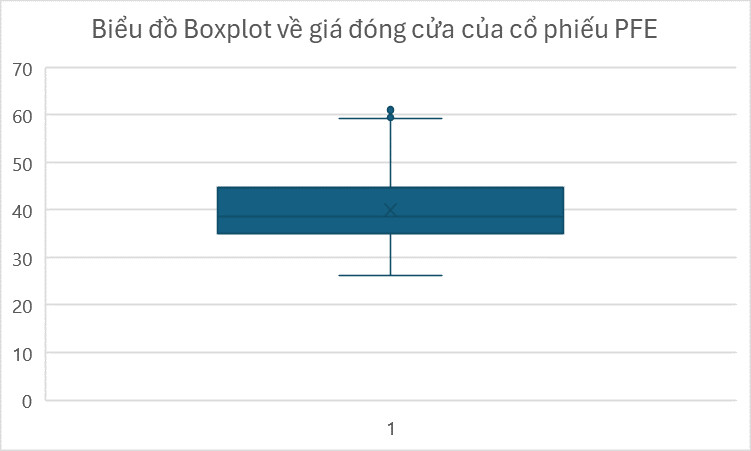
\includegraphics[width=1\textwidth]{Image/PFE_Boxplot.jpg}
    \caption{Biểu đồ Box Plot giá đóng cửa của PFE}
    \label{fig:1}
    \end{minipage}
    \hfill
    \begin{minipage}{0.23\textwidth}
    \centering
    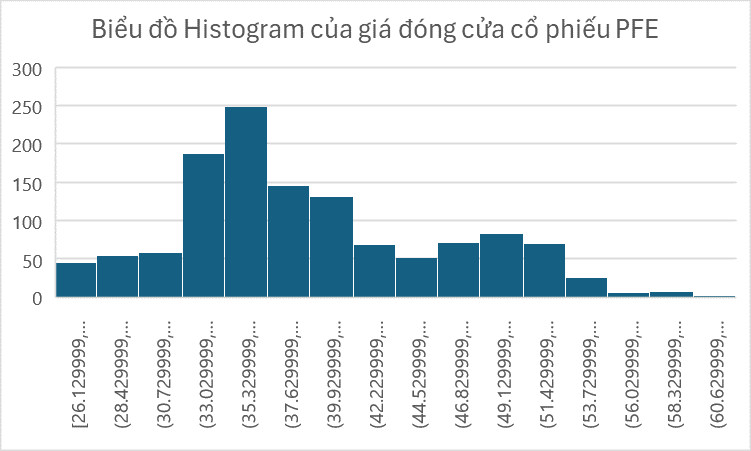
\includegraphics[width=1\textwidth]{Image/PFE_Histogram.jpg}
    \caption{Biểu đồ Histogram giá đóng cửa của PFE}
    \label{fig:2}
    \end{minipage}
\end{figure}
- Giá trị Skewness dương cho thấy phân phói dữ liệu lệch nhẹ về bên phải.

- Giá trị Kurtosis này nhỏ hơn 0 cho thấy phân phối có độ nhọn thấp hơn bình thường.

- Biểu đồ Histogram cho thấy tần suất xuất hiện của giá cổ phiếu có giá trị từ 35.33 đến 37.63 là nhiều nhất.

- Biểu đồ Boxplot cho thấy dữ liệu cổ phiếu PFE có giá trị ngoại lai nằm ngoài giá trị max và độ phân tán ít.

Để quá trình thực nghiệm đạt hiệu quả tốt nhất, chúng tôi sử dụng một số công cụ bao gồm: Google Colab - Colaborator hay còn gọi là Google Colab, là một sản phẩm từ Google Research, nó cho phép chạy các dòng lệnh code python qua trình duyệt. Có thể sử dụng tài nguyên máy tính để chạy nhanh hơn như CPU tốc độ cao, GPUs, TPUs, …Visual Studio Code - Là một trình soạn thảo mã nguồn mở gọn nhẹ nhưng có khả năng vận hành mạnh mẽ trên 3 nền tảng là Windows, Linux và macOS được phát triển bởi Microsoft. Bên cạnh đó, chúng tôi sử dụng một số thư viện trong quá trình thực nghiệm như: numpy, pandas, matplotlib, scikit-learn, keras, minmaxscaler,…
\subsection{CÁC ĐỘ ĐO CHẤT LƯỢNG}
Chúng tôi đánh giá hiệu suất của các mô hình dự báo bằng ba chỉ số chính: Sai số trung bình bình phương (RMSE), Sai số trung bình tuyệt đối (MAE), và Sai số trung bình tuyệt đối phần trăm (MAPE), đảm bảo kiểm thử chính xác và toàn diện.

RMSE (Sai số trung bình bình phương): RMSE đại diện cho căn bậc hai của sai số trung bình bình phương giữa các giá trị dự báo và quan sát được. Nó thường được sử dụng trong phân tích hồi quy và dự báo, đặc biệt là khi độ chính xác là quan trọng. Giá trị RMSE thấp hơn chứng tỏ mức độ chính xác cao hơn trong các dự đoán của mô hình.

MAE (Sai số trung bình tuyệt đối): MAE đo lường độ lớn trung bình của sai số trong một tập hợp các dự đoán, bất kể chúng có phải là sự đánh giá cao hơn hay thấp hơn so với giá trị thực tế. Nó đánh giá hiệu quả của một mô hình hồi quy bằng cách tính trung bình khác biệt tuyệt đối giữa các giá trị dự đoán và các giá trị thực tế.

MAPE (Sai số trung bình tuyệt đối phần trăm): MAPE đánh giá độ chính xác dưới dạng phần trăm và được xác định là trung bình khác biệt phần trăm tuyệt đối giữa các giá trị dự đoán và các giá trị thực tế cho mỗi khoảng thời gian.

Công thức của RMSE:
\[RMSE=\sqrt{\sum_{i=1}^{n} \frac{(\hat{y_i}-y_i )^2}{n} }\]

Công thức của MAE:
\[MAE=\frac{1}{n}  \sum_{i=1}^{n} |y_i-\hat{y_i} |\]

Công thức của MAPE:
\[MAPE=\frac{1}{n}  \sum_{i=1}^{n} |\frac{y_i-\hat{y_i}}{y_i}|\]
Trong đó:\\
	\indent\textbullet\ \(n\) số lượng quan sát trong dữ liệu.\\
	\indent\textbullet\ \(y_i\)  giá trị thực tế của điểm dữ liệu thứ i.\\
	\indent\textbullet\ \(\hat{y_i}\) giá trị dự đoán của điểm dữ liệu thứ i.

\section{PHƯƠNG PHÁP}
\subsection{LINEAR REGRESSION}
Trong lĩnh vực thống kê, Linear Regression là một phương pháp dùng để xác định mối quan hệ giữa một biến phụ thuộc có giá trị số và một hoặc nhiều biến độc lập.

Khi chỉ có một biến độc lập, chúng ta gọi là hồi quy tuyến tính đơn giản (Simple Linear Regression). Trong trường hợp có nhiều biến độc lập, ta gọi là hồi quy tuyến tính đa biến (Multiple Linear Legression)

Simple Linear Regression được mô tả qua công thức: \\

\( y = \beta_0 + \beta_1 x + \varepsilon \) \\

Trong đó:\\
	\indent\textbullet\ \(y\) : biến phụ thuộc (dependent variable) cần dự đoán.\\
	\indent\textbullet\ \(x\) : biến độc lập (independent variable) được sử dụng để dự đoán giá trị của y.\\
        \indent\textbullet\ $\beta_0$ : hệ số góc (intercept) của đường hồi quy, đại diện cho giá trị dự đoán của y khi x = 0.\\
        \indent\textbullet\ $\beta_1$ : hệ số hồi quy (regression coefficient), đại diện cho mức độ thay đổi của y dựa trên mỗi đơn vị thay đổi của x.\\
        \indent\textbullet\ $\varepsilon$: lỗi ngẫu nhiên (random error), biểu thị sự không thể tránh khỏi của mô hình trong việc mô phỏng dữ liệu thực tế.
\subsection{ARIMA}
Trong một mô hình ARIMA, giá trị tương lai của một biến được giả định là một hàm tuyến tính của một số quan sát quá khứ cộng với các lỗi ngẫu nhiên. Hàm tuyến tính này dựa trên ba thành phần tham số: tự hồi quy (AR), tích hợp sai phân (I) và trung bình trượt (MA). Mô hình ARIMA có thể được ký hiệu là ARIMA(p, d, q), trong đó p là số lượng thành phần tự hồi quy, d là số lượng sự khác biệt không mùa và q là số lượng lỗi dự báo trễ trong phương trình dự đoán. Giá trị tương lai của một biến trong ARIMA được biểu thị như sau:\\

\( y(t) = \varnothing_0 + \varnothing_1 y_{t-1} + \varnothing_2 y_{t-2} + \ldots + \varnothing_p y_{t-p} + \varepsilon_t - \theta_1 \varepsilon_{t-1} - \theta_2 \varepsilon_{t-2} - \ldots - \theta_q \varepsilon_{t-q} \) \\

Trong đó:\\
	\indent\textbullet\ \(y_t\) : giá trị thực tế.\\
	\indent\textbullet\ $\varepsilon_t$: sai số ngẫu nhiên tại thời điểm t.\\
        \indent\textbullet\ $\varnothing_i$ và $\varnothing_j$ : các hệ số.\\

\section{THỰC NGHIỆM}
\subsection{THỰC NGHIỆM TRÊN BỘ BA DỮ LIỆU}
\begin{figure}[H]
    \centering
    \begin{minipage}{0.5\textwidth}
    \centering
    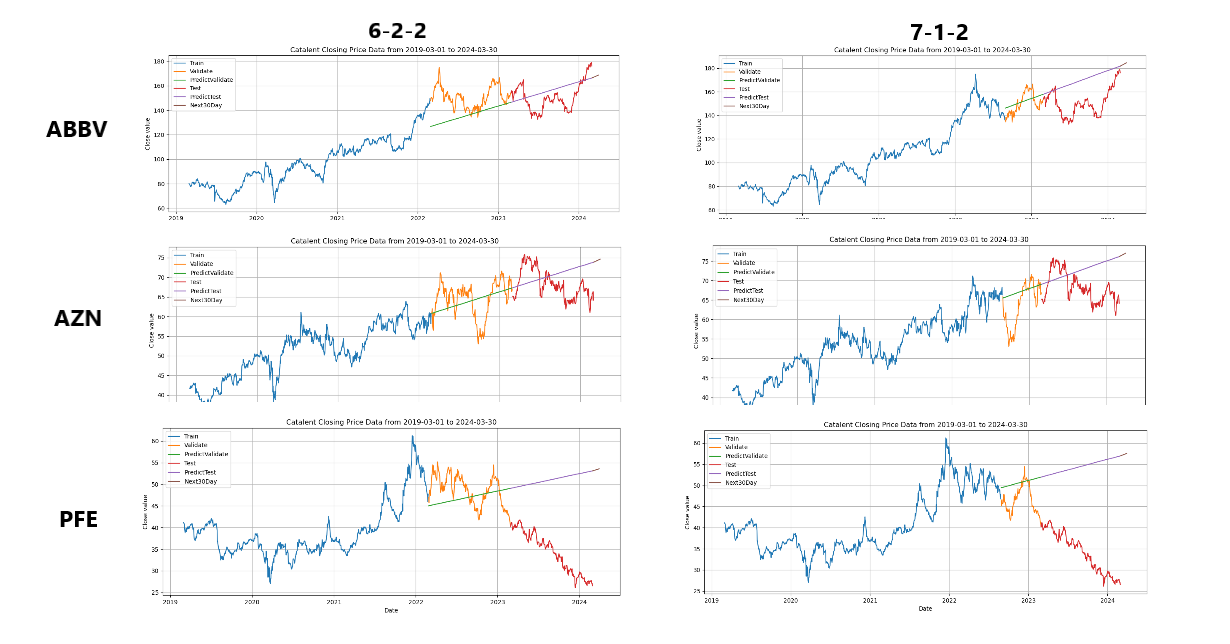
\includegraphics[width=1\textwidth]{Image/LinearRegression.png}
    \caption{Kết quả thực nghiệm Linear Regression}
    \label{fig:1}
    \end{minipage}
\end{figure}
\begin{figure}[H]
    \centering
    \begin{minipage}{0.5\textwidth}
    \centering
    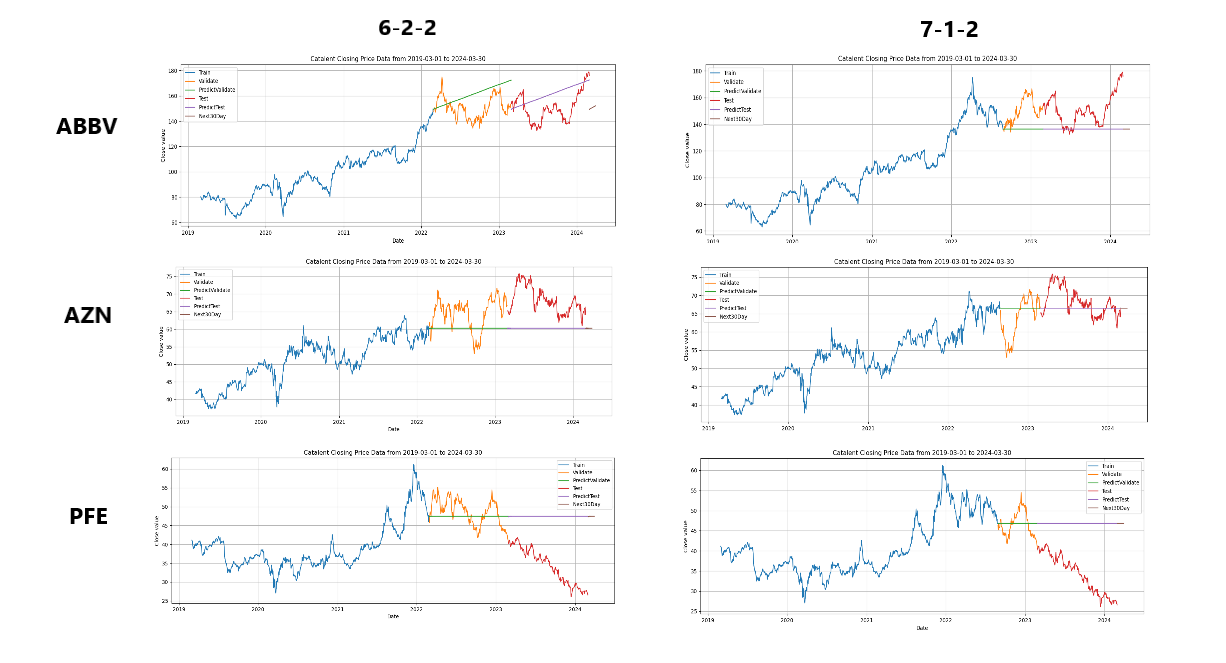
\includegraphics[width=1\textwidth]{Image/ARIMA.png}
    \caption{Kết quả thực nghiệm ARIMA}
    \label{fig:1}
    \end{minipage}
\end{figure}
\begin{figure}[H]
    \centering
    \begin{minipage}{0.5\textwidth}
    \centering
    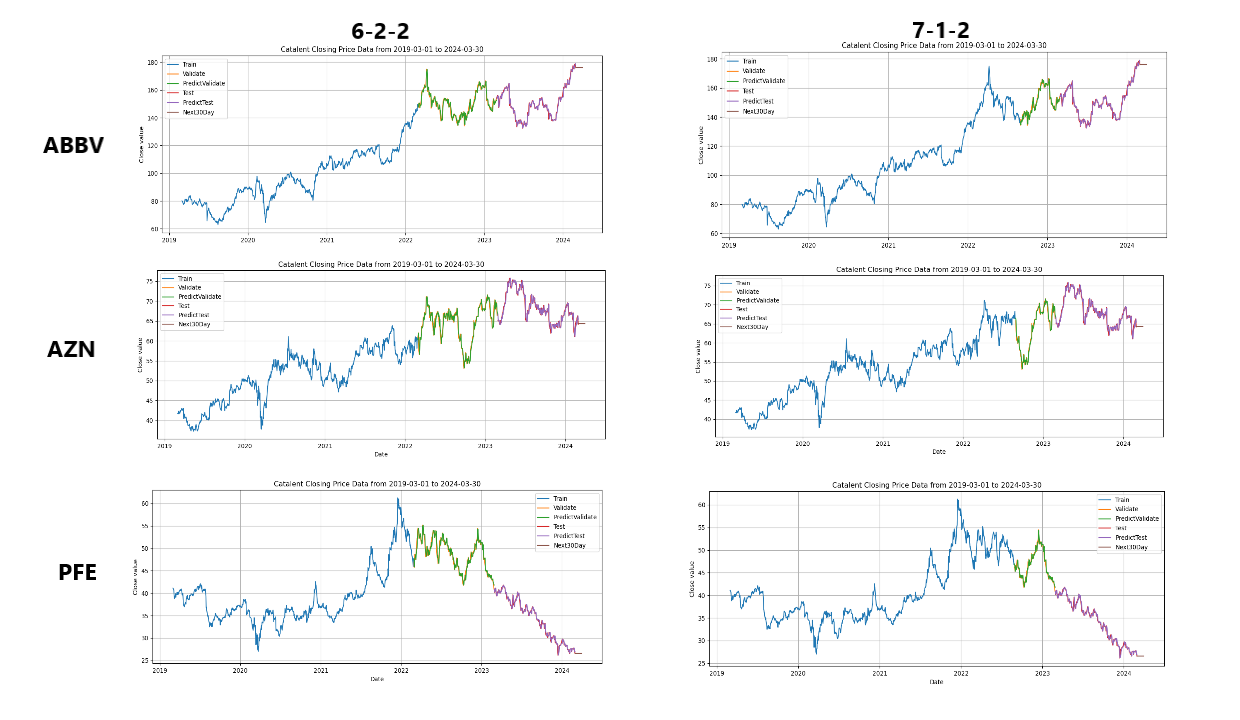
\includegraphics[width=1\textwidth]{Image/ETS.png}
    \caption{Kết quả thực nghiệm ETS}
    \label{fig:1}
    \end{minipage}
\end{figure}
\begin{figure}[H]
    \centering
    \begin{minipage}{0.5\textwidth}
    \centering
    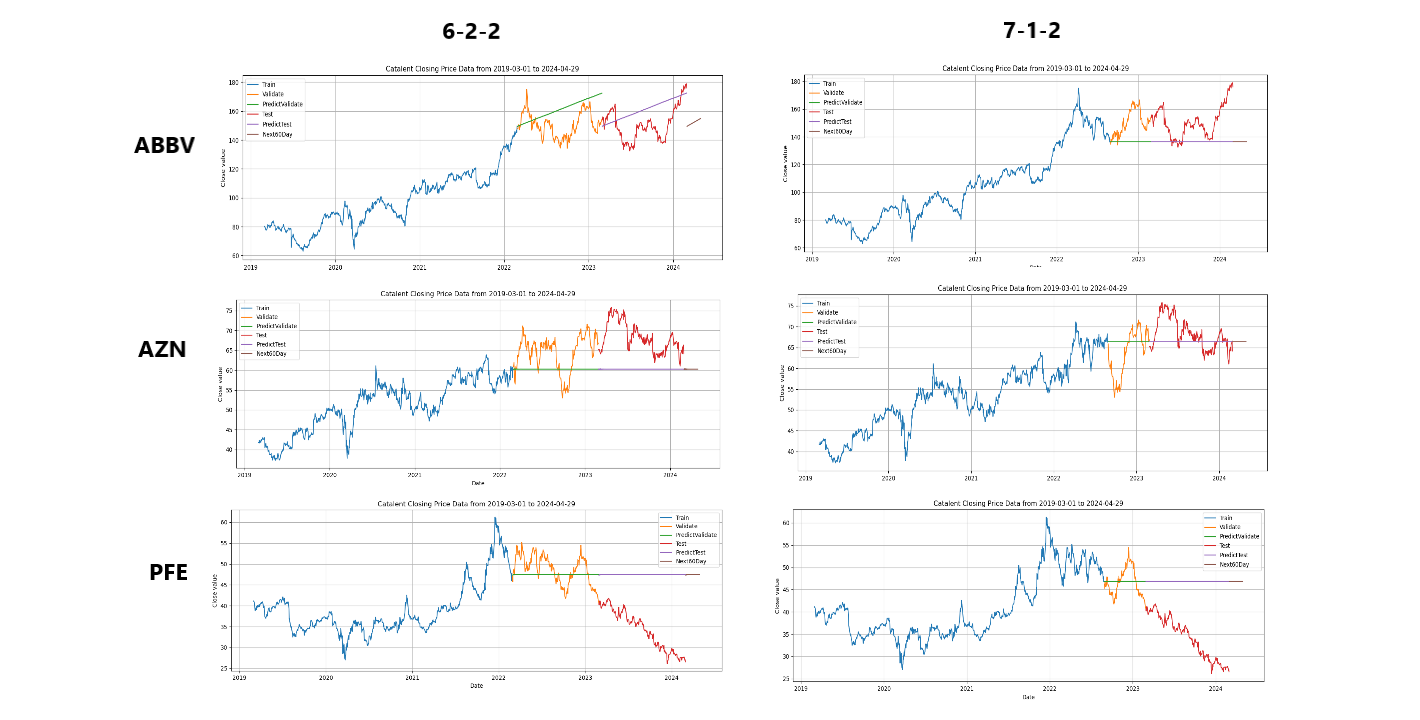
\includegraphics[width=1\textwidth]{Image/meta learning.png}
    \caption{Kết quả thực nghiệm Meta learning}
    \label{fig:1}
    \end{minipage}
\end{figure}
\begin{figure}[H]
    \centering
    \begin{minipage}{0.5\textwidth}
    \centering
    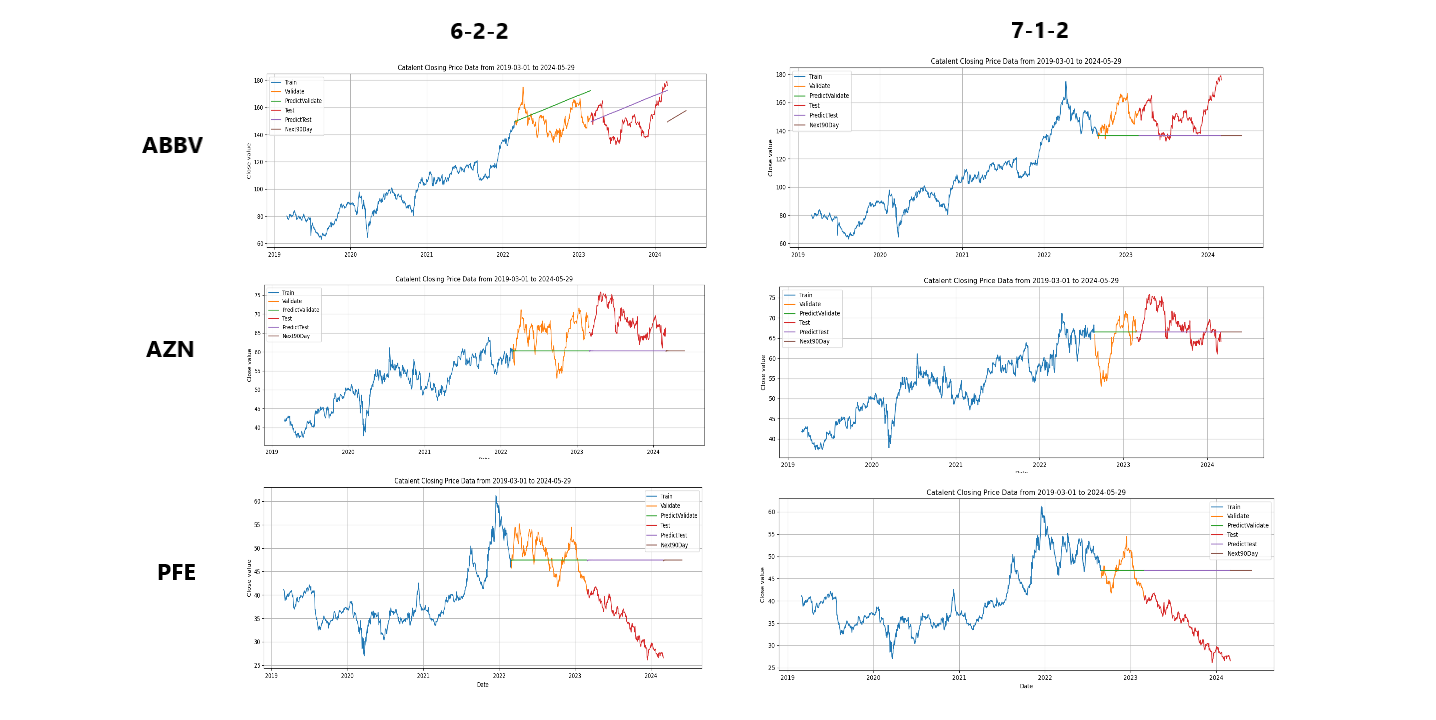
\includegraphics[width=1\textwidth]{Image/Fuzzy for predict times series.png}
    \caption{Kết quả thực nghiệm Fuzzy for predict times series}
    \label{fig:1}
    \end{minipage}
\end{figure}

\begin{thebibliography}{00}
\bibitem{b1} Zou Xiaowu, Wang Zidong, Li Qi, Sheng Weiguo ``Integration of residual network and convolutional neural network along with various activation functions and global pooling for time series classification'' ,2019. [Online]. Link: https://www.sciencedirect.com/science/article/abs/pii/S0925231219311506
\bibitem{b2} Guolin Ke, Qi Meng, Thomas Finley ``LightGBM: A Highly Efficient Gradient Boosting Decision Tree'' ,2017. [Online]. Link: https://proceedings.neurips.cc/paper\_files/paper/2017/file/...
\bibitem{b3} Mária Lakatos, Sebastian Lerch, Stephan Hemri, Sándor Baran ``Comparison of multivariate post-processing methods using global ECMWF ensemble forecasts'' ,2023. [Online]. Link: https://rmets.onlinelibrary.wiley.com/doi/full/10.1002/qj.4436
\bibitem{b4} S. Julier and J. Uhlmann, “New extension of the Kalman filter to nonlinear systems,” Proceedings of SPIE, Jul. 1997, doi: 10.1117/12.280797.
\bibitem{b5} Gang Liu, Fuyuan Xiao, ... (2020) ``A Fuzzy Interval Time-Series Energy and Financial Forecasting Model Using Network-Based Multiple Time-Frequency Spaces and the Induced-Ordered Weighted Averaging Aggregation Operation''.[Online]. Link: https://ieeexplore.ieee.org/abstract/document/8988162
\bibitem{b6} Gururaj, V., Shriya, V. R., & Ashwini, K. (2019). Stock market prediction using linear regression and support vector machines. Int J Appl Eng Res, 14(8), 1931-1934.
\bibitem{b7} Disha, R. A., & Waheed, S. (2022). Performance analysis of machine learning models for intrusion detection system using Gini Impurity-based Weighted Random Forest (GIWRF) feature selection technique. Cybersecurity, 5(1), 1-20
\bibitem{b8} A. A. Ariyo, A. O. Adewumi and C. K. Ayo, "Stock Price Prediction Using the ARIMA Model," 2014 UKSim-AMSS 16th International Conference on Computer Modelling and Simulation, Cambridge, UK, 2014, pp. 106-112, doi: 10.1109/UKSim.2014.67.
\bibitem{b9} A. Meyler, G. Kenny and T. Quinn, “Forecasting Irish Inflation using ARIMA Models”, Central Bank of Ireland Research Department, Technical Paper, 3/RT/1998.
\bibitem{b10} Roondiwala, M., Patel, H., & Varma, S. (2017, April). Predicting Stock Prices Using LSTM. IJSC publishing.
\bibitem{b11}	Yongqiong Zhu. 2020. Stock price prediction using the RNN model. 2020 International Conference on Applied Physics and Computing (ICAPC 2020). IOP Publishing.

\end{thebibliography}
\vspace{12pt}
\color{red}
\end{document}
